\documentclass{article}%[final]
\setcounter{secnumdepth}{3}
% if you need to pass options to natbib, use, e.g.:
% \PassOptionsToPackage{numbers, compress}{natbib}
% before loading nips_2016
%
% to avoid loading the natbib package, add option nonatbib:
% \usepackage[nonatbib]{nips_2016}

%\usepackage{nips_2016}

% to compile a camera-ready version, add the [final] option, e.g.:
%\usepackage[final]{nips_2016}
\usepackage{amsmath}
\usepackage[utf8]{inputenc} % allow utf-8 input
\usepackage[T1]{fontenc}    % use 8-bit T1 fonts
\usepackage{hyperref}       % hyperlinks
\usepackage{url}            % simple URL typesetting
\usepackage{booktabs}       % professional-quality tables
\usepackage{amsfonts}       % blackboard math symbols
\usepackage{nicefrac}       % compact symbols for 1/2, etc.
\usepackage{microtype}      % microtypography
\usepackage{float}
\usepackage{amssymb}
\usepackage{amsthm}
\usepackage{color,soul}
\usepackage{amsmath}
\usepackage{algorithm}
\usepackage[noend]{algpseudocode}
\usepackage[margin=1.5in]{geometry}
\usepackage[english]{babel}
\usepackage{graphicx}
\usepackage{longtable}

\newtheorem{theorem}{Theorem}[section]
\newtheorem{lemma}[theorem]{Lemma}
\newtheorem{proposition}[theorem]{Proposition}
\newtheorem{corollary}[theorem]{Corollary}
\theoremstyle{definition}
\newtheorem{definition}{Definition}[section]

%\theoremstyle{definition}
%\newtheorem{definition}{Definition}[section]


\makeatletter
\def\BState{\State\hskip-\ALG@thistlm}
\makeatother

\title{Implementing the Collapsed Gibbs Sampler for Latent Dirichlet Allocation}

% The \author macro works with any number of authors. There are two
% commands used to separate the names and addresses of multiple
% authors: \And and \AND.
%
% Using \And between authors leaves it to LaTeX to determine where to
% break the lines. Using \AND forces a line break at that point. So,
% if LaTeX puts 3 of 4 authors names on the first line, and the last
% on the second line, try using \AND instead of \And before the third
% author name.

\author{
  Steve Bronder \\
  %Quantitative Methods of the Social Sciences\\
  %Columbia University\\
  %New York City, NY 10027 \\
  \texttt{sab2287@columbia.edu} \\
  %% examples of more authors test etst
   \and
   Antonio Moretti \\
   %Department of Computer Science \\
   %Columbia University\\
   %New York City, NY 10027 \\
   \texttt{am4134@columbia.edu} \\
  %% \AND
  %% Coauthor \\
  %% Affiliation \\
  %% Address \\
  %% \texttt{email} \\
  %% \And
  %% Coauthor \\
  %% Affiliation \\
  %% Address \\
  %% \texttt{email} \\
  %% \And
  %% Coauthor \\
  %% Affiliation \\
  %% Address \\
  %% \texttt{email} \\
}

\begin{document}
% \nipsfinalcopy is no longer used

\maketitle

\begin{abstract}
  %The purpose of this document is to 
  Latent Dirichlet Allocation is a two stage hierarchical clustering process that is typically fit through MCMC or variational inference. In this note we describe how the collapsed Gibbs sampler is derived and implemented, including the method of integrating out multinomial parameters as an example of Rao-Blackwellization. This allows for all samples to be drawn from simple conditional distributions while also supporting the update of each topic distribution after each word is assigned to a particular topic. We demonstrate our implementation in Fortran by performing posterior inference on a collection of documents from JSTOR. We review a few open problems and discuss heuristics to check rates of convergence.  %With regards to Topic Models, integrating out the Multinomial parameters allows for all samples to be drawn from simple discrete distributions while also supporting a Gibbs sampling scheme such that each model is updated after each word is assigned to a particular topic. After theoretical explanations are given, an example of Latent Dirichlet Analysis with a Collapsed Gibbs Sampler will be implemented in Python.
  \end{abstract}

\section{Introduction}
Topic models are a family of unsupervised machine learning methods for summarizing and organizing large collections of documents. Topic models aim to mimic the writing process in which an author draws upon a set of topics based on the focus of the narrative. Words represent various topics and provide clues about the underlying themes that comprise the document. Introduced by Blei in 2003,  Latent Dirichlet Allocation (LDA) has become a widely popular topic model for text processing due to its simplicity \cite{Blei:2003:LDA:944919.944937}. The same model is derived in 2000 by Pritchard for isolating microbial species using genotype data \cite{Pritchardetal2000}. Pritchard's motivation is to describe the genome of an individual or species as a mixture of various populations. At its core, LDA is a two level Bayesian heirarchical model for clustering with hidden factors. Formally, a topic is defined as a hidden probability distribution over a fixed vocabulary. Documents are modeled as mixtures of topic distributions, which in turn are modeled as distributions over words. This two stage hierarchical structure supports a soft rather than a hard assignment of each document to multiple topics where words are the only variables observed. \nocite{10.2307/2685208,citeulike:6744178} 
%\nocite{Heinrich04parameterestimation}

%\paragraph{Outline} 
In this note we illustrate how to implement the collapsed Gibbs sampler for LDA. The rest of this document is organized as follows. We introduce the LDA model in Section~\ref{sec:ldamodel}. In Section~\ref{sec:inference} we discuss the process of learning parameters and the challenge of posterior inference to motivate the MCMC approach. Section~\ref{sec:gibbs} describes the collapsed Gibbs sampler for LDA as an application of Rao-Blackwellization including a brief summary of the Hammersley-Clifford theorem. We discuss our implementation and experimental results in Section~\ref{sec:implementation}. Section~\ref{sec:conclusion} concludes by briefly addressing a few open questions. Mathematical derivations and basic results are provided for completeness along with output and figures in Section~\ref{sec:appx}.

%\hl{Started with a more academic description of topic models}

%Imagine you hand a participant in a study one hundred printed Wikipedia articles and instruct them to sort the Wikipedia articles into six different topics. The participant would read through each article, grabbing associations such as Greek mythology and World War II, and slowly sort through the papers, at times moving some articles from one topic to the other, until the participant felt certain he had separated the articles into their respective topic. The goal of topic modeling is to formalize this abstract clustering process through statistical models that, much like our participant, give us some level of certainty about what topics a particular group of documents will be centered around.

\section{LDA Model}
\label{sec:ldamodel}
In order to state the model we will introduce the notation below. Following Carpenter \cite{Carpenter10integrating}, let $K$ be the number of topics and let $M$ be the number of documents. Let $N_m$ be the number of words in the $m$th document and let $J$ be the distinct number of words in the corpus. Let  $W_{m,n}$ be the observed document term matrix where rows represent documents, columns represent words and the components are the counts of the $n$th word in the $m$th document. Let $Z_{m,n} \in 1:K$ be the topic to which the word of $W_{m,n}$ is assigned. Let $\theta_m \in [0, 1]^K$ be the topic distribution for the $m$th document and $\phi_k \in [0, 1]^J$ be the word distribution for the $k$th topic. The hyperparameter $\alpha \in \mathbb{R}^K$ is a vector of prior counts for topics in documents. Similarly $\beta \in \mathbb{R}^J$ is a vector of prior counts for words in a given topic.
%(\hl{Describe the model as derived in Griffiths or the Blei paper from 2003... }) 
LDA is defined by the following generative model.
\begin{enumerate}
    \item For each topic $k$ draw a word distribution: 
    \begin{enumerate}
        \item $\phi_k \sim Dirichlet(\beta)$
    \end{enumerate}
    \item For each document $m$: 
        \begin{enumerate}
        \item $\theta_m \sim Dirichlet(\alpha)$
        \item For each of the $n$ words in $m$:
        \begin{enumerate}
            \item $z_{m,n} \sim Mult(\theta_m) $
            \item $w_{m,n} \sim Mult(\phi_{z_{m,n}}) $ 
        \end{enumerate}
        \end{enumerate}
\end{enumerate}
The joint distribution of the graphical model factorizes as products of the conditional distributions:
\begin{equation}
    p(\theta | \alpha)p(z|\theta) p(w|z, \phi)p(\phi | \beta)
\end{equation}
Define $c_{k,m,j}$ to be the count for the number of times word $j$ is assigned to topic $k$ in document $m$:
\[ c_{k,m,j} = \sum\limits_{n=1}^{Nm}I\Big(z_{m,n} = k \ \& \ w_{m,n} = j \Big) \]
Note that we can marginalize the distribution of counts over any of the three variables $k, m$ and $j$. For example,
\[ c_{k,m,*} = \sum\limits_{j=1}^{J}c_{k,m,j} \]
It will be useful to recast the above using linear algebra. Let NMZ be a matrix of M rows and Z columns whose components denote the number of times document M and topic Z occur together. Similarly, let NZW represent a matrix of Z rows and W columns whose components denote the number of times topic Z and word W interact. Marginalizing the above with respect to W and Z give vectors NM and NZ respectively. 

\section{Posterior Inference for LDA}
\label{sec:inference}
The learning task for LDA is to compute the posterior distribution which is the conditional distribution of hidden variables given the observations:
\begin{equation}
P(\theta, z, \phi | w, \alpha, \beta) \propto \prod\limits_{k=1}^{K}p(\phi_k | \beta) \prod\limits_{m=1}^{M}p(\theta_m|\alpha)\prod\limits_{n=1}^{N}p(z_{m,n}|\theta_m)p(w_{m,n}|z_{m,n},\phi_k)
\end{equation}
Recall the first two terms are Dirichlet. The third term represents a draw of the topic assignment $\theta_d$ for each of the $N_m$ words in the document. The last term represents the likelihood of drawing a word given the joint distribution of observations and hidden variables. It is easy to see that evaluating the above presents computational challenges. Consider for simplicity that we are dealing with one document where the topics $\phi_k$ are fixed. The per document posterior is then proportional to the following.
\begin{align}
p(\theta|\alpha)\prod\limits_{n=1}^{N}p(z_n|\theta)p(w_n|z_n,\phi_k) \\
\intertext{In order to ensure that the above is normalized it is necessary to compute the evidence.}
\int_\theta p(\theta|\alpha)\prod\limits_{n=1}^{N}\sum\limits_{z=1}^{K}p(z_n|\theta)p(w_n|z_n,\phi_k)d\theta
\end{align}
The above is a hypergeometric function shown by Dickey to be intractable \cite{10.2307/2288131}. One solution is to move the summation outside the integral to obtain the form of the evidence below:
\begin{equation}
\sum\limits_{z=1}^{K}\int_\theta p(\theta|\alpha)\prod\limits_{n=1}^{N}p(z_n|\theta)p(w_n|z_n,\phi_k) d\theta
\end{equation}
The simplified form is equivalent to the sum of $N^k$ tractable Dirichlet integrals, however when k is reasonably large it is not practical to compute the solution exactly. Even without or multiple documents, we are forced to compute an exponential number of Dirichlet integrals. Two solutions include the use of approximate inference algorithms such as MCMC via the Gibbs sampler or variational methods such as mean field variational inference~\cite{NIPS2006_3113}. 
%\hl{Why is the posterior distribution intractable? Motivate MCMC... }
%In order to compute the parameters in LDA we must evaluate the posterior distribution:
%\begin{equation}
    %\int \int p(\theta | \alpha)p(z|\theta) p(w|z, \phi)p(\phi | \beta) d\theta d\phi
%    p(\theta, z | w, \alpha, \beta) = \frac{P(\theta, z, w | \alpha, \beta)}{P(w|\alpha, \beta)}
%\end{equation}
%\begin{equation}
%P(w|\alpha, \beta) = \frac{\Gamma(\sum_i \alpha_i)}{\prod_i \Gamma(\alpha_i)} \int \Big( \prod\limits_{i=1}^{k} \theta^{\alpha_i -1}\Big) \Big(\prod\limits_{n=1}^{N} \sum\limits_{i=1}^{k} \prod\limits_{j=1}^{J} (\theta_i \phi_{ij})^{w^j} \Big) d\theta
%\end{equation}

\section{The Gibbs Sampler}
\label{sec:gibbs}
MCMC methods exploit the fundamental theorem of Markov chains to sample from an intractible distribution such as (2). The MCMC approach is to design an irreducible, aperiodic and positive recurrent chain whose stationary distribution is the posterior distribution of interest. We will use the space of all configurations of hidden variables to represent the state space of a Markov chain. Recall that the Gibbs sampler approach is to iteratively sample from the distribution of one hidden variable at a time conditioned on the observations and the current state of each of the other hidden variables. After a suitable burn-in period, collecting samples will result in a Monte Carlo estimate of the posterior. 

A naive sampler would condition on all of the hidden variables, however it is possible to integrate out the multinomial parameters for a faster mixing chain. We summarize the necessary derivations in detail in the Appendix. We note here that by using conditional expectations we can improve the variance of the Monte Carlo estimate. 
\begin{equation}
    Var(\mathbb{E}[\delta(X)|Y]) \leq Var(\delta(X))
\end{equation}
We review some basic properties of the Gibbs sampler and Rao-Blackwellization below. %We wish to show that the support of the joint distribution $f$ is the Cartesian product of marginal distributions. 
\nocite{Robert:2005:MCS:1051451}
\begin{definition}
The positivity condition for a joint distribution $f(X_1,\cdots, X_p)$ with marginal densities $f_{X_i}(x_i)$ is satisfied if the following holds: $f_{X_i}(x_i) > 0$ for all $(X_1,\cdots, X_p)$ implies that $f(X_1,\cdots, X_p) > 0$.
\end{definition}
\begin{theorem}[Hammersley-Clifford]
\label{thm:hc}
Suppose that $(X_1,\cdots,X_d)$ satisfies the positivity condition with joint pdf $f(X_1,\cdots, X_p)$. For all $(Y_1, \cdots Y_p) \in supp(f)$
\begin{equation}
f(X_1,\cdots, X_p) \propto \prod\limits_{i=1}^{P} \frac{f_{X_i} | X_{-i}(X_i | X_1, \cdots X_{i-1}, Y_{i+1}, \cdots Y_p)}{f_{X_i} | X_{-i}(Y_i | X_1, \cdots X_{i-1}, Y_{i+1}, \cdots Y_p)}
\end{equation}
\end{theorem}
\begin{proof}
\begin{align}
    f(X_1, \cdots, X_{p-1}, X_p) &= f_{X_p}(X_p | X_1, \cdots X_{p-1})f(X_1, \cdots X_{p-1}) \\
\intertext{Similarly we have that}
    f(X_1, \cdots, X_{p-1}, Y_p) &= f_{X_p}(Y_p | X_1, \cdots X_{p-1})f(X_1, \cdots X_{p-1}) \\
\intertext{By equation (5) we can write the following.}
    f(X_1,\cdots, X_p) &= f(X_1,\cdots, X_{p-1}) f_{X_p}(X_p | X_1, \cdots X_{p-1})\\
\intertext{Rewrite the joint distribtion on the RHS using equation (6).}
    &= f(X_1,\cdots, X_{p-1}, Y_p) \frac{f_{X_p}(X_p | X_1, \cdots X_{p-1})}{f_{X_p}(Y_p | X_1, \cdots X_{p-1})}\\
\intertext{Repeating this process of rewriting the joint in terms of conditionals:}
&= \cdots \\
&= f(X_1,\cdots, X_p)\frac{f_{X_p}(X_p | Y_1, \cdots Y_p)}{f_{X_p}(Y_p | Y_1, \cdots Y_{p})} \cdots \frac{f_{X_p}(X_p | X_1, \cdots X_{p-1})}{f_{X_p}(Y_p | X_1, \cdots X_{p-1})}
\end{align}
\end{proof}
\noindent The Hammersley-Clifford theorem specifies when a distribution can be factorized in terms of cliques. In order to make use of Rao-Blackwellization for the Gibbs sampler, we require the joint distribution to be uniquely specified by conditional distributions. 
%Theorem \ref{thm:hc} demonstates that the conditional distributions we are interested in sampling from are non-zero. We require like the joint distribution to be uniquely specified by conditional distributions, however this is by construction from the graphical model. Sampling from the conditional distributions then generates a Markov chain whose stationary distribution is the posterior of interest. 
\begin{lemma}
The transition probability matrix of the Gibbs sampler is 
\begin{align}
\nonumber    K(x^{(t-1)},x^{(t)}) &= f_{X_1|X_{-1}}(x_1 | x_1^{t-1}, \cdots x_{p}^{t-1}) \times f_{X_2 | X_{-2}}(x_2^t | x_1^{t}, x_3^{t-1} \cdots x_{p}^{t-1}) \\
    &\qquad \times \cdots \times f_{X_p | X_{-p} }(x_p^t | x_1^{t}, x_{p_1}^{t}, \cdots x_{p}^{t-1})
\end{align}
\end{lemma}
\begin{proof}
\begin{align}
P(X^t \in \mathcal{X} | X^{t-1} = x^{t-1}) &= \int_\mathcal{X} f_{X_t | X_{t-1}}(x^t | x^{t-1})dx^t \\
\nonumber &= \int_\mathcal{X} f_{X_1|X_{-1}}(x_1 | x_1^{t-1}, \cdots x_{p}^{t-1}) \times f_{X_2 | X_{-2}}(x_2^t | x_1^{t}, x_3^{t-1} \cdots x_{p}^{t-1}) \\
    &\qquad \qquad \qquad \times \cdots \times f_{X_p | X_{-p} }(x_p^t | x_1^{t}, x_{p_1}^{t}, \cdots x_{p}^{t-1}) dx^t
\end{align}
\end{proof}
%\hl{Brief review of MCMC and gibbs sampling... }
There are two rules that are required to create an MCMC sampler, one to propose how to move from $x$ to $y$, and another rule to accept that move as the new position. In the context of the Gibbs sampler, suppose the stationary distribution \textbf{$X$}$=(X_1,\ldots,X_d)$ is 
\begin{equation}
    \pi(X_1,\ldots,X_d) = g(X_1,X_2,\ldots,X_d)/ \kappa
\end{equation}
\noindent where $\kappa$ is a normalizing constant. Given the current value $\mathbf{x}=(x_1,x_2,\ldots,x_d)$, for the next move we follow the steps below.
\begin{enumerate}
    \item Assign $J\sim U(1,2,\ldots,n)$.
    \item Sample $X_j$ with the proposal distribution $\pi(\tilde{x}_J|x_1,\ldots,x_{J-1},x_{J+1},\ldots,x_d)$ where $\tilde{x}_J$ is our proposed move from the first rule. 
\end{enumerate}
\noindent Unlike some MCMC samplers, the Gibbs sampler accepts this next move with probability one. The update equation for the onditional distribution used for Gibbs sampling is given below according to (32) derived in the Appendix:
\begin{equation}
p(z_{a,b}|z_{-(a,b)},y,\alpha,\beta) = \frac{\nicefrac{(\alpha_{z_{a,b}}+ c+_{z_{a,b},a,*}^{-(a,b)})\times(\beta_{y_{a,b}}+c_{z_{a,b},a,*}^{-(a,b)})}{(J \times \beta_j + c_{z_{a,b},*,*}^{-(a,b)})}}{\sum_{k=1}^{K}\nicefrac{(\alpha_{z_{a,b}}+ c+_{z_{a,b},a,*}^{-(a,b)})\times(\beta_{y_{a,b}}+c_{z_{a,b},a,*}^{-(a,b)})}{(J \times \beta_j + c_{z_{a,b},*,*}^{-(a,b)})}}
\end{equation}

\section{Implementation and Experimental Results}
\label{sec:implementation}
The implementation of the collapsed Gibbs sampler is relatively simple and described in detail in Algorithm 1. High level pseudocode can be found in Heinrich~\cite{Heinrich04parameterestimation}. During initialization, a random topic is assigned for each word of each document and the corresponding counts in the matrices NMZ, NM, NZ and NZW are incremented. The Gibbs sampler itself proceeds as follows. For each iteration, document, and every word in the document, matrices representing the counts by document and topic as well as word and topic are decremented. Then, the probability of moving to another topic is selected, and a realization is made from a multinomial distribution as the new topic for that word. The new topic is then added to document and word count matrices. Due to the large amount of looping necessary in the algorithm an implementation was developed in Fortran 95 as higher level languages such as Python or matlab could not satisfy time constraints when working with large matrices\footnote{The code and Python notebook associated with this research can be found at \url{https://github.com/stevo15025/topicmodelpy}}.

Data was gathered on 200 journal entries submitted to the Journal of the American Statistical Association. Word counts for journal entries were made available by JSTOR's Data for Research program. With five topics selected, the topic model ran over the document term matrix for 30,000 iterations, burning in the first 18,000 iterations. Performing Geweke's \cite{Geweke92evaluatingthe} diagnostic test on the likelihood, as seen in figure 1, with the first window being at the tenth percentile and the second window at the fiftieth yielded a t-score of 1.504, enough to feel satisfied that the model has converged after this many iterations. Investigating the chain using Heidel's criterion \cite{doi:10.1287/opre.31.6.1109}  we receive a p-value for the stationarity test of .191 and pass the half-width test, which means we do not reject the null hypothesis of stationarity and have enough samples to accurately estimate the mean. 

\begin{table}[!ht]
\centering
\caption{The top 10 words for each topic}
\begin{tabular}{rlllll}
  \hline
 & Topic 1 & Topic 2 & Topic 3 & Topic 4 & Topic 5 \\ 
  \hline
1 & inconsistent & hildreth & adapted & zin & presumably \\ 
  2 & ext & affects & snedecor & harvey & stop \\ 
  3 & algebra & ath & exposition & pooled & paired \\ 
  4 & advantages & lag & gets & eliminate & indicators \\ 
  5 & benjamin & requiring & averaging & diagram & exception \\ 
  6 & thompson & heuristic & bls & singular & computable \\ 
  7 & continues & classified & mcleod & load & locally \\ 
  8 & sectors & alternatively & anything & lhs & markets \\ 
  9 & width & cal & marvin & carlin & empirically \\ 
  10 & originally & lot & payments & friedman & adler \\ 
   \hline
\end{tabular}
\end{table}

Table one shows the top 10 words for each topic. We can see that each topic tends to follow a pattern in the statistical literature. For instance, topic three is associated with words about approximation while topic four requires linear algebra and singular value decomposition. We can also see topic five may hold words associated with econometrics.

Tables two through five in the appendix show the articles that have the highest probability of being in each topic. Note how topic one seems to be comprised of topics on sampling procedures and estimating significance. One thing we see in all topics is how frequent back matter, letters to the editor, and book reviews matter. This may be due to these papers in particular journals summing up large breaths of what was popular at that particular time in statistical literature. Also note that some articles such as "Exact Distribution of the Sum of Independent Identically Distributed Discrete Random Variables" appear multiple times. This is due to the probabilistic nature of the topic model algorithm. As each article has a certain probability of being in a topic, some articles will be general enough to fit in one or more topics.





\section{Conclusion and Future Work}
\label{sec:conclusion}
%\hl{outline a few open questions / areas of active research wrt Gibbs sampler}

One important area of research that has not seen much focus is dealing with memory issues when study convergence properties for these large models. At every iteration of a topic model you receive back two matrices, one of size documents by topics and another by topics and words. If you have one thousand documents and thirty thousand words it is very easily to run into memory out of bounds errors as only 10 iterations can take up a significant portion of memory. Implementing chunking methods as well as online models for the convergence procedure, for instance an online ARMA model, to reduce memory consumption would allow researchers to investigate convergence properties of these models much more clearly.

Another open question about MCMC methods concerns whether or not theoretical bounds can be constructed that address how long to run the chain. Rates of convergence between the transition kernel and the stationary distribution $K^n(x,y) \rightarrow \pi$ are usually measured by total variation distance:
\begin{equation}
\|K_x^n - \pi \|_{TV} = \frac{1}{2}\sum_y | K^n(x,y) - \pi(y)| = \max_{A \subseteq \mathcal{X}} |K^n(x,A) - \pi(A) |
\end{equation}
A natural question is whether or not we can derive eigenvalue bounds on rates of convergence by using a reversible chain Gibbs sampler. Note that the Gibbs sampler implemented here is not reversible. That is, $\pi(x)K(x,y) \neq \pi(y)K(y,x)$. Liu (1995) describes the following reversible chain:
\begin{enumerate}
    \item Sample an index $j$ uniformly form the distribution on $\{1, \cdots, p\}$
    \item Sample $X_j^{(t)} \sim f_{X_j |X_{-j}}(\cdot | X_1^{(t-1)},\cdots, X_{j-1}^{(t-1)},  X_{j+1}^{(t-1)}, \cdot  X_{p}^{(t-1)})$ setting $X_i^{(t)}=X_i^{(t-1)}$ $\forall i \neq j$.
\end{enumerate}
For the reversible case, $Kg(x) = \sum g(y)K(x,y)$ and so the Markov kernel is a self adjoint operator $\langle Kg, h\rangle = \langle g, Kh\rangle$. We can then factorize the transition kernel using a spectral decomposition. Let $\psi_i$ be the eigenvectors and $\beta_i$ be the corresponding eigenvalues such that $K\psi_i = \beta\psi_i$ for $0 \leq i \leq |\mathcal{X}|-1$:
\begin{equation}
K(x,y) = \pi(y) \sum\limits_{i=0}^{|\mathcal{X}|-1}\beta_i\psi_i(x)\psi_i(y) \qquad K^n(x,y) = \pi(y) \sum\limits_{i=0}^{|\mathcal{X}|-1}\beta_i^n\psi_i(x)\psi_i(y)
\end{equation}
Diaconis shows that we can derive an eigenvalue bound using the Cauchy-Schwartz inequality:
\begin{equation}
4\|K^n_x - \pi \|^2_{TV} \leq \sum\limits_{y}^{} \frac{(K^n(x,y) - \pi(y))^2}{\pi(y)} = \sum\limits_{i=0}^{|\mathcal{X}|-1}\beta_i^{2n}\psi_i^2(x)
\end{equation}
Several other heuristics exist for MCMC convergence rates and NLP models. Two examples the perplexity score which is a function of entropy and quantifies how well a distribution fits a sample $2^{H(p)} = 2^{-\sum p(x) log p(x)}$, and the Gelman-Rubin test. In future work we wish to explore various criteria for model convergence. 

One approach that is not discussed here is that of variational inference. The idea here is to select a family of distributions over the hidden variables and to find corresponding parameters that make the variational parameters as close as possible to the posterior. This often involves minimizing the KL divergence between the two distributions. Naturally there is a nice parallel and intuitive analogy with the EM algorithm. A good discussion of this approach is given by Hoffman~\cite{Hoffman:2013:SVI:2502581.2502622}. LDA has also been expanded in an attempt to automatically learn topic heirarchies to model increasingly complex phenomena. Several approaches have been proposed that draw on the theory of the distribution of random partitions known as Chinese restuarant processes. For an interesting discussion of the above the reader is referred to the following work by Paisley~\cite{DBLP:journals/pami/PaisleyWBJ15} and Blei~\cite{Blei04hierarchicaltopic}.

%\small
\bibliography{mybib}{}
\bibliographystyle{plain}
\clearpage
\section{Appendix}
\label{sec:appx}
\subsection{Integrating out Multinomial Parameters}
\begin{align}
    &\int \int p(\theta | \alpha)p(z|\theta) p(w|z, \phi)p(\phi | \beta) d\theta d\phi \\
    \intertext{The joint distribution factorizes based on dependencies specified by the graphical model.}
    &=\int p(\theta | \alpha)p(z|\theta)d\theta \int p(w|z, \phi)p(\phi | \beta) d\phi \\
    \intertext{Take the product over documents and topics and replace the conditional probabilities with the Multinomial and Dirichlet distributions.}
    &= \prod_{m=1}^M \int \frac{\Gamma(\sum \alpha_k)}{\prod \Gamma(\alpha_k)} \prod_{k=1}^{K} \theta^{\alpha_k-1}\prod_{n=1}^{Nm} \theta^{c_{k,m,*}} d\theta \prod_{k=1}^{K} \int \frac{\Gamma(\sum \beta_j)}{\prod \Gamma(\beta_j)} \prod_{j=1}^{J} \phi^{\beta_j-1}\prod_{m=1}^{M} \prod_{n=1}^{Nm} \phi^{c_{k,*,j}} d\phi \\
    \intertext{Rewrite the above exploiting the congucacy between prior and posterior.} 
        &= \prod_{m=1}^M \int \frac{\Gamma(\sum \alpha_k)}{\prod \Gamma(\alpha_k)} \prod_{k=1}^{K} \theta^{\alpha_k + c_{k,m,*}-1} d\theta \prod_{k=1}^{K} \int \frac{\Gamma(\sum \beta_j)}{\prod \Gamma(\beta_j)} \prod_{j=1}^{J} \phi^{\beta_j + c_{k,*,j}-1} d\phi \\
    \intertext{Note that both integrals are unnormalized Dirichlets. Multiply by the normalization constant and its reciprocal to cancel both integrals as they evaluate to 1 by definition.}
        %&= \prod_{m=1}^M \int \frac{\Gamma(\sum \alpha_k)}{\prod \Gamma(\alpha_k)} \prod_{k=1}^{K} \theta^{\alpha_k + c_{k,m,*}-1} d\theta \prod_{k=1}^{K} \int \frac{\Gamma(\sum \beta_j)}{\prod \Gamma(\beta_j)} \prod_{j=1}^{J} \phi^{\beta_j + c_{k,*,j}-1} d\phi \\
        &= \prod_{m=1}^M \frac{\Gamma(\sum \alpha_k)}{\prod \Gamma(\alpha_k)}\frac{\prod \Gamma(\alpha_k + c_{k,m,*})}{\Gamma(\sum \alpha_k + c_{k,m,*})} \prod_{k=1}^{K} \frac{\Gamma(\sum \beta_j)}{\prod \Gamma(\beta_j)} \frac{\prod \Gamma(\beta_j + c_{k,*,j})}{\Gamma(\sum \beta_j + c_{k,*,j}) } \\
    \intertext{Drop terms that do not depend on the distribution over counts $c_{k,m,j}$}
        &\propto \prod_{m=1}^M \frac{\prod \Gamma(\alpha_k + c_{k,m,*})}{\Gamma(\sum \alpha_k + c_{k,m,*})} \prod_{k=1}^{K} \frac{\prod \Gamma(\beta_j + c_{k,*,j})}{\Gamma(\sum \beta_j + c_{k,*,j}) } \\
    \intertext{Split the product over documents and topics including/excluding the $(a,b)$th component.}
        &= \prod_{m \neq a}^{}\frac{\prod \Gamma(\alpha_k + c_{k,m,*})}{\Gamma(\sum \alpha_k + c_{k,m,*})}\frac{\prod \Gamma(\alpha_k + c_{k,a,*})}{\Gamma(\sum \alpha_k + c_{k,a,*})} \times \prod_{k=1}^k \frac{\prod_{j\neq y_{a,b}}^{}\Gamma(\beta_j + c_{k,*,j}) \Gamma(\beta_{y_{ab}} + c_{k,*,y_{a,b}})}{\Gamma(\sum \beta_j + c_{k,*,j}) } \\
    \intertext{Drop terms that do not depend on current position (a,b)}
        &\propto \frac{\prod_{k=1}^{K}\Gamma(\alpha_k + c_{k,a,*})}{\Gamma(\sum_{k=1}^{K}\alpha_k + c_{k,a,*})} \prod_{k=1}^{K}\frac{\Gamma(\beta_{y_{ab}}+ c_{k,*,y_{ab}})}{\Gamma(\sum \beta_j + c_{k,*,j})} \\
    \intertext{Split the product over topics including/excluding the $c^{a,b}$th component}
        &\propto \frac{\prod_{k \neq z_{ab}}^{} \Gamma(\alpha_k + c_{k,a,*}^{-(a,b)}) \times \Gamma(\alpha_{z_{a,b}}+ c_{z_{a,b},a,*}^{-(a,b)})}{\Gamma(1+ \sum \alpha_k + c_{k,a,*}^{-(a,b)})} \\
        \nonumber &\qquad \qquad \times \prod_{k\neq z_{a,b}}^{K}\frac{\Gamma(\beta_{y_{a,b}}+ c_{k,*,y_{a,b}}^{-(a,b)})}{\Gamma(\sum \beta_j + c_{k,*,j})} \frac{\Gamma(\beta_{y_{a,b}}+c_{z_{a,b},*,y_{a,b}}^{-(a,b)}+1)}{\Gamma(1+\sum \beta_j + c_{z_{a,b},*,j}^{-(a,b)})} \\
    \intertext{Use the fact that that $\Gamma(x+1) = x\Gamma(x)$}
        &= \frac{\prod_{k \neq z_{a,b}}^{} \Gamma(\alpha_k + c_{k,a,*}^{-(a,b)})\Gamma(\alpha_{z_{a,b}}+c_{z_{a,b},a,*}^{-(a,b)})(\alpha_{z_{a,b}}+c_{z_{a,b},a,*}^{-(a,b)})}{\Gamma(1+\sum \alpha_k + c_{k,a,*}^{-(a,b)})} \\
        \nonumber &\qquad \qquad \times \prod_{k\neq z_{a,b}}^{} \frac{\Gamma(\beta_{y_{a,b}}+c_{k,*,y_{a,b}}^{-(a,b)})}{\Gamma(\sum \beta_j + c_{k,*,j})} \frac{\Gamma(\beta_{y_{a,b}}+c_{z_{a,b},*,y_{a,b}}^{-(a,b)})}{\Gamma(\sum \beta_j + c_{z_{a,b},*,j}^{-(a,b)})} \frac{(\beta_{y_{a,b}}+c_{z_{a,b},*,y_{a,b}}^{-(a,b)})}{\sum (\beta_j + c_{z_{a,b},*,j}^{-(a,b)})} \\
    \intertext{Combine the $\Gamma$ terms back into the product:}
        &= \frac{\prod_{k=1}^{K}\Gamma(\alpha_k + c_{k,a,*}^{-(a,b)})(\alpha_{z_{a,b}}+c_{z_{a,b},*,y_{a,b}}^{-(a,b)})}{\Gamma(1+\sum \alpha_k + c_{k,a,*}^{-(a,b)})} \\
        \nonumber &\qquad \qquad \qquad \qquad \times \prod_{k=1}^{K}\frac{\Gamma(\beta_{y_{a,b}}+c_{k,*,y_{a,b}}^{-(a,b)})}{\Gamma(\sum \beta_j + c_{z_{a,b},*,j}^{-(a,b)})}\frac{(\beta_{y_{a,b}}+ c_{z_{a,b},*,y_{a,b}}^{-(a,b)})}{\sum(\beta_j + c_{z_{a,b},*,j}^{-(a,b)})} \\
    \intertext{Drop the topic denominator and general product terms which are constant:}
        %&= \frac{\prod_{k=1}^{k}\Gamma(\alpha_k + c_{k,a,*}^{-(a,b)})\times (\alpha_{z_{a,b}} + c_{z_{a,b},a,*}^{-(a,b)})}{\Gamma(1+\sum \alpha_k + c_{k,a,*}^{-(a,b)})} \\
        %\nonumber &\qquad \qquad \times \prod_{k=1}^{K}\frac{\Gamma(\beta_{y_{a,b}}+c_{k,*,y_{a,b}}^{-(a,b)})}{\Gamma(\sum \beta_j + c_{k,*,j})} \frac{\beta_{y_{a,b}} +c_{z_{a,b},*,y_{a,b}}^{-(a,b)}}{\sum(\beta_j + c_{z_{a,b},*,j}^{-(a,b)})} \\
    %\intertext{}
        &\propto \frac{(\alpha_{z_{a,b}}+ c+_{z_{a,b},a,*}^{-(a,b)})\times(\beta_{y_{a,b}}+c_{z_{a,b},a,*}^{-(a,b)})}{\sum(\beta_j + c_{z_{a,b},*,j}^{-(a,b)})} = \frac{(\alpha_{z_{a,b}}+ c_{z_{a,b},a,*}^{-(a,b)})\times(\beta_{y_{a,b}}+c_{z_{a,b},a,*}^{-(a,b)})}{\sum(\beta_j) + c_{z_{a,b},*,*}^{-(a,b)}}
\end{align}
The conditional distribution used for Gibbs sampling is given by normalizing the result above:
\begin{equation}
p(z_{a,b}|z_{-(a,b)},y,\alpha,\beta) = \frac{\nicefrac{(\alpha_{z_{a,b}}+ c_{z_{a,b},a,*}^{-(a,b)})\times(\beta_{y_{a,b}}+c_{z_{a,b},a,*}^{-(a,b)})}{(J \times \beta_j + c_{z_{a,b},*,*}^{-(a,b)})}}{\sum_{k=1}^{K}\nicefrac{(\alpha_{z_{a,b}}+ c_{z_{a,b},a,*}^{-(a,b)})\times(\beta_{y_{a,b}}+c_{z_{a,b},a,*}^{-(a,b)})}{(J \times \beta_j + c_{z_{a,b},*,*}^{-(a,b)})}}
\end{equation}

\subsection{The Gamma, Beta and Dirichlet Redux}
Euler would introduce the useful function below. 
\[\Gamma(x) = \int\limits_{0}^{\infty}t^{x-1}e^{-t}dt = 2\int\limits_{0}^{\infty}u^{2x-1}e^{-u^2}du \]
Substituting $t = u^2$ and evaluating $x = 1/2$ gives the Euler-Poisson integral. 
\[\Gamma(\nicefrac{1}{2}) = 2\int\limits_{0}^{\infty}e^{-u^2}du = \sqrt{\pi}\]
Using integration by parts it is easy to see $\Gamma(x+1) = x\Gamma(x)$ and thus $\Gamma(x+1) = x!$ when $x$ is an integer. 
\begin{align*}
\Gamma(n) &= \int\limits_{0}^{\infty}e^{-x}x^{n-1}dx \\
\Gamma(n+1) &= \int\limits_{0}^{\infty}e^{-x}x^{n}dx \\
\intertext{Let $u=x^n, du = nx^{n-1}$, $dv=e^{-x}$ and $v=-e^{-x}$}
&= -x^{n}e^{-x}\Big|_0^{\infty} - \int\limits_{0}^{\infty}-e^{-x}nx^{n-1}dx \\
&= n \int\limits_{0}^{\infty}e^{-x}x^{n-1}dx = n\Gamma(n) \\
%\end{align*}
\intertext{Euler found that by using the Gamma function we can define the Beta function:}
\frac{\Gamma(x)\Gamma(y)}{\Gamma(x+y)} &= B(x,y) = \int\limits_{0}^{1}t^{a-1} (1-t)^{b-1}dt \\
\intertext{The beta is constructed using Gamma functions of two variables. The Gamma function can be used to derive the Beta. Perform the substitution $t = sin^2(\theta)$:}
%\begin{proofs}
%\begin{align*}
B(x,y) &= \int\limits_{0}^{1}t^{x-1}(1-t)^{y-1}dt 
\\&= \int \limits_{0}^{\pi/2}sin(t)^{2x-1}cos(t)^{2y-1}dt = B(y,x)\\
\Gamma(x)\Gamma(y) &= 4 \int\limits_{0}^{\infty}u^{2x-1}e^{-u^2}du\int\limits_{0}^{\infty}v^{2y-1}e^{-v^2}dv \\
&= 4 \int\limits_{0}^{\infty}\int\limits_{0}^{\infty}e^{-(u^2+v^2)}u^{2x-1}v^{2y-1}du dv \\
%\end{align*}
%\end{proofs}
\intertext{Let $u = r \ cos (\theta)$  and $v = r \ sin (\theta)$:}
%\begin{align*}
&= 4 \int\limits_{0}^{\infty}\int\limits_{0}^{\pi/2}e^{-r^2}r^{2(x+y)-1}cos^{2x-1}(\theta)sin^{2y-1}(\theta) dr d\theta \\
&= 2 \int\limits_{0}^{\infty}r^{2(x+y)-1}e^{-r^2}dr \times 2\int\limits_{0}^{\pi/2}cos^{2x-1}(\theta)sin^{2y-1}(\theta) d\theta \\
\Gamma(x)\Gamma(y)&= \Gamma(x+y)B(y,x) \\
\frac{\Gamma(x)\Gamma(y)}{\Gamma(x+y)} &= B(y,x)
\end{align*}
\qed

%\end{proofs}
Recall that the Dirichlet is constructed from Gamma functions of $d$ variables:
\begin{equation*}
p(x|\alpha) = \frac{\Gamma(\sum_i \alpha_i)}{\prod_i \Gamma(\alpha_i)}\prod\limits_{i=1}^{d}x_i^{\alpha_i-1}
\end{equation*}
The Dirichlet distribution is the conjugate prior to the Multinomial. Note the similar functional form. 
\begin{align*}
posterior &\propto likelihood \times prior \\
&= \frac{\Gamma(n+1)}{\prod \Gamma(x_i+1)} \prod\limits_{i=1}^{K}p_i^{x_i}\frac{\Gamma(\sum \alpha_i)}{\prod \Gamma(\alpha_i)}\prod\limits_{}^{}x_i^{\alpha_i-1} \\
&\propto \prod_{y_i}\prod_{j=1}^{K}p_j^{y_i^{(j)}}\prod\limits_{j=1}^{K} p_j^{\alpha_j-1}\\
&= \prod\limits_{j=1}^{K} p_j^{\alpha_j-1 + \sum y_i^{(j)}}\\
&= Dir(a_j + \sum y_i)
\end{align*}
The posterior is again a Dirichlet random variable whose new parameters are increased by the sum of the multinomial parameters.


\begin{figure}[h]
  \caption{Likelihood Over Sampled Iterations}
  \centering
    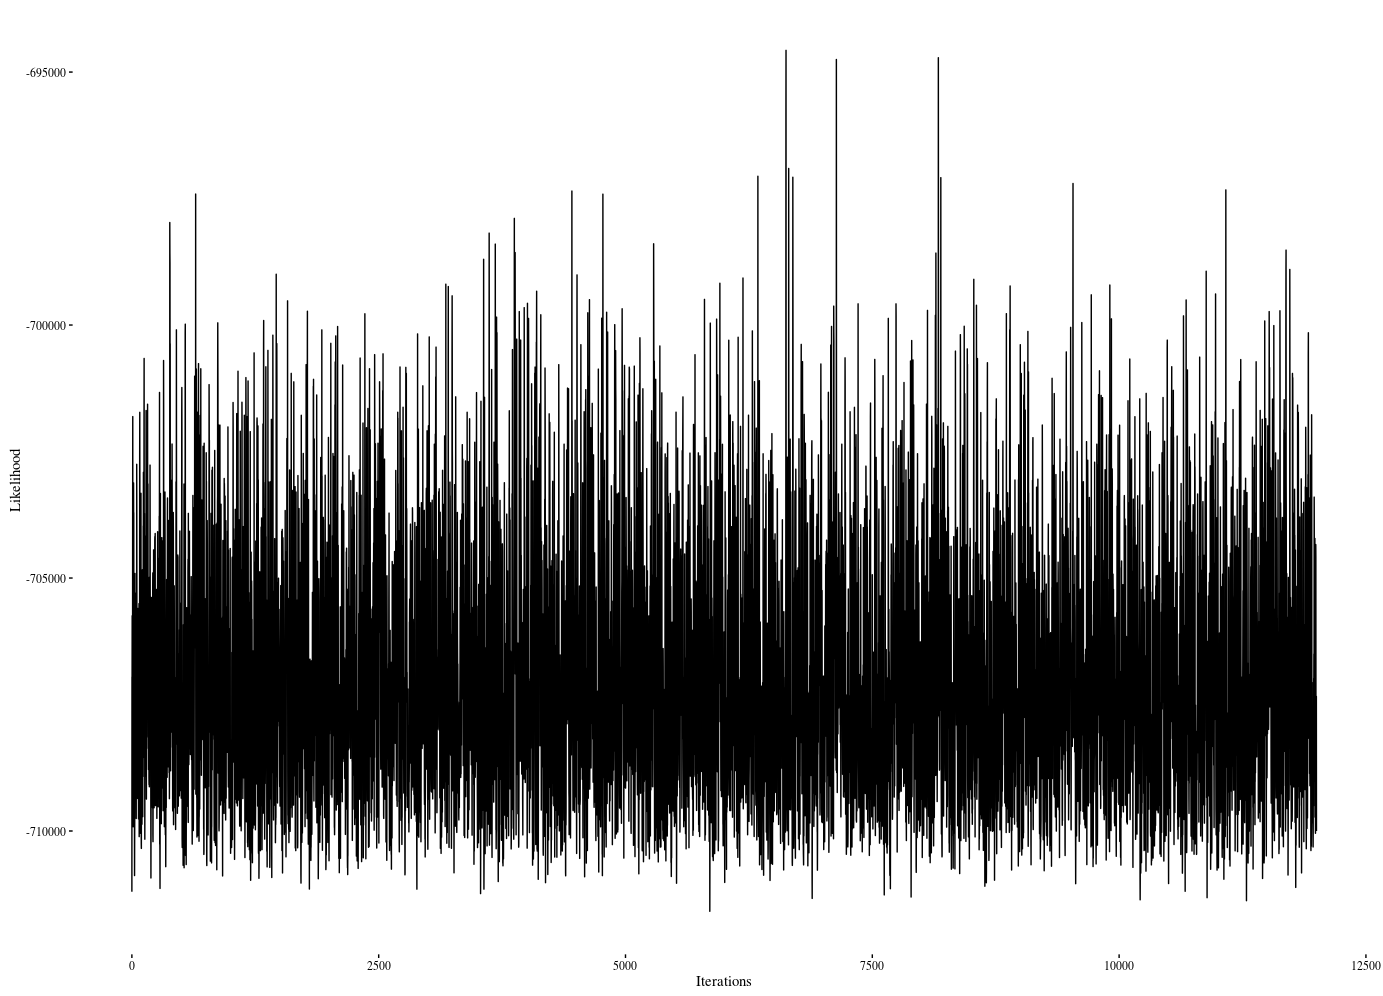
\includegraphics[width=1\textwidth]{Likelihood}
\end{figure}

\begin{algorithm}
\caption{Topic Model Procedure}\label{euclid}
\begin{algorithmic}[1]
\State \Comment{ Define Variables}
\State integer :: m,n, top\_size, Z, gg, kk, i, j, ll, nn
\State integer, dimension(n,m) :: matrix
\State integer, dimension(ntopics,n) :: NZW
\State integer, dimension(ntopics,m) :: NZM
\State integer, dimension(ntopics) :: NZ
\State integer, dimension(m) :: NM
\State integer, intent(in) :: ntopics, max\_iter
\State integer, dimension(top\_size) :: topics
\State integer, dimension(ntopics) :: genZ
\State real, dimension(ntopics) :: p\_z
\State real,intent(in) :: alpha, beta
\Procedure{Collapsed Gibbs Sampler}{}
\State \For {i in 1:iterations}
\State kk = 1
\State  \For {j in 1:len(Documents)}
\State   \For {ll in 1:len(words)}
\If {$\text{matrix}(ll,j) == 0$} Next
\EndIf
\State     \For {nn in 1:matrix(ll,j)}
\State Z = topics(kk)
\State \Comment{Decrement DocumentTopic and WordTopic matrices}
\State NZM(Z,j) = NZM(Z,j) - 1
\State NM(j) = NM(j) - 1
\State NZW(Z,ll) = NZW(Z,ll) - 1
\State NZ(Z) = NZ(Z) - 1
\State
\State vocab = count which(matrix(:,j) != 0)
\State
\State p\_z = $\frac{\text{(NZM(:,j) + alpha) $\times$ (NZW(ll,:) + beta)}}{\text{NZ + vsize $\times$ beta}}$
\State
\State p\_z = p\_z / sum(p\_z)
\State \Comment{ Generate Realization from Multinomial Distribution}
\State call GENMUL(1,p\_z,ntopics, genZ)
\State Z = which(genZ == 1)
\State  topics(kk) = Z
\State kk = kk + 1
\State \Comment{Increment DocumentTopic and WordTopic matrices}
\State NZM(Z,j) = NZM(Z,j) + 1
\State NM(j) = NM(j) + 1
\State NZW(Z,ll) = NZW(Z,ll) + 1
\State NZ(Z) = NZ(Z) + 1
\State    \EndFor
\State   \EndFor
\State  \EndFor
\State \EndFor
\State Phi = NZM / sum(NZM,by='cols')
\State Theta = NZW / sum(NZW,by='rows')
\EndProcedure
\end{algorithmic}
\end{algorithm}


\begin{table}[ht]
\centering
\caption{Articles in Topic One}
\begin{tabular}{rl}
  \hline
 & Topic One \\ 
  \hline
1 & A Test for Significance in a Unique Sample \\ 
  2 & Volume Information \\ 
  3 & Letter to the Editor \\ 
  4 & Selective Service's Medical Statistics Program \\ 
  5 & Analysis of Coarsely Grouped Data from the Lognormal Distribution \\ 
  6 & Sub-Balanced Data and the Mixed Analysis of Variance \\ 
  7 & On Variance Estimation With Imputed Survey Data: Rejoinder \\ 
  8 & Exact Distribution of the Sum of Independent Identically Distributed Discrete Random Variables \\ 
  9 & Back Matter \\ 
  10 & Note on Estimating Significance of a Number of Samples \\ 
   \hline
\end{tabular}
\end{table}


\begin{table}[ht]
\centering
\caption{Articles in Topic Two}
\begin{tabular}{rl}
  \hline
 & Topic Two \\ 
  \hline
1 & Bayesian Approach to Life Testing and Reliability Estimation \\ 
  2 & Inadmissibility of the Usual Scale Estimate for a Shifted Exponential Distribution \\ 
  3 & [List of Book Reviews] \\ 
  4 & Progress of Work in the Census Bureau \\ 
  5 & Nomographs for ... Differences Between the Frequencies of Events in Two Contrasted Series or Groups \\ 
  6 & Estimating Population Size with Exponential Failure \\ 
  7 & Missing Observations in Multivariate Statistics. III: Large Sample Analysis of Simple Linear Regression \\ 
  8 & Self-Calibrating Priors Do Not Exist: Comment \\ 
  9 & Wage Rates and Per Capita Productivity \\ 
  10 & A Method of Appraising Short-Term Forecasts \\ 
   \hline
\end{tabular}
\end{table}


\begin{table}[ht]
\centering
\caption{Articles in Topic Three}
\begin{tabular}{rl}
  \hline
 & Topic Three \\ 
  \hline
1 & Committee on Nominations \\ 
  2 & Back Matter \\ 
  3 & Miscellaneous Notes \\ 
  4 & On Non-Negative Quadratic Unbiased Estimation of Variance Components \\ 
  5 & Corrections: Comment on "Semi-Parametric Nonlinear Mixed-Effects Models and Their Application" \\ 
  6 & Notes About Authors \\ 
  7 & [List of Book Reviews] \\ 
  8 & Self-Calibrating Priors Do Not Exist: Comment \\ 
  9 & The Revised Index of the Volume of Trade \\ 
  10 & Calculation of Chi-Square for Complex Contingency Tables \\ 
   \hline
\end{tabular}
\end{table}

\begin{table}[ht]
\centering
\caption{Articles in Topic Four}
\begin{tabular}{rl}
  \hline
 & Topic Four \\ 
  \hline
1 & Exact Distribution of the Sum of Independent Identically Distributed Discrete Random Variables \\ 
  2 & Notes About Authors \\ 
  3 &  A Stochastic Analysis of the Size Distribution of Firms \\ 
  4 &  Bayesian Approach to Life Testing and Reliability Estimation \\ 
  5 & Index of Book Reviewers \\ 
  6 & Note on Estimating Significance of a Number of Samples \\ 
  7 & Diversity as a Concept and its Measurement: Rejoinder \\ 
  8 & [List of Book Reviews] \\ 
  9 & Committee on Nominations \\ 
  10 & A Two-Stage Minimax Procedure for Selecting the Normal Population with the Smallest Variance \\ 
   \hline
\end{tabular}
\end{table}


% latex table generated in R 3.2.3 by xtable 1.8-0 package
% Mon May 16 15:50:35 2016

\begin{table}[ht]
\centering
\caption{Articles in Topic Five}
\begin{tabular}{rl}
  \hline
 & Topic 5 \\ 
  \hline
1 &  Exact Distribution of the Sum of Independent Identically Distributed Discrete Random Variables \\ 
  2 & [List of Book Reviews] \\ 
  3 &  A Stochastic Analysis of the Size Distribution of Firms \\ 
  4 & Committee on Nominations \\ 
  5 & Notes About Authors \\ 
  6 & Letter to the Editor \\ 
  7 & A Test for Extreme Value Domain of Attraction \\ 
  8 & Estimates of Bounded Relative Error for the Ratio of Variances of Normal Distributions \\ 
  9 & Progress of Work in the Census Bureau \\ 
  10 & Continuous Sequential Testing of a Poisson Process to Minimize the Bayes Risk \\ 
   \hline
\end{tabular}
\end{table}


%\subsection{Fundamental Theorem of Markov Chains}
%\hl{Review some basic properties of markov chains including ergodic thm}

%Let $S$ be the state space of a markov chain.
%\theoremstyle{definition}
%\begin{definition}%{Irreducible}
%A markov chain is \textit{irreducible} if the following holds:
%\[ \forall i, j \in S, \exists \ m < \infty \ s.t. \ P(X_{n +m} = j | X_n = i) > 0 \]
%\end{definition}

%\[\text{The posterior form } p(\theta | \mathcal{D}, \mathcal{M}) \text{ is the same as the prior } p(\theta | \mathcal{M}) \]

%%%%%%%%%%%%%%
%Some papers for reading:

%What is LDA?
%\begin{center}
%  \url{http://u.cs.biu.ac.il/~89-680/darling-lda.pdf}
%\end{center}

%Integrating out multinomial parameters.
%\begin{center}
%  \url{https://lingpipe.files.wordpress.com/2010/07/lda3.pdf}
%\end{center}

%Latent Dirichlet Allocation (Original Paper)
%\begin{center}
%  \url{https://www.cs.princeton.edu/~blei/papers/BleiNgJordan2003.pdf}
%\end{center}

%Gibbs Sampling for the Uninitiated.
%\begin{center}
%  \url{https://www.umiacs.umd.edu/~resnik/pubs/LAMP-TR-153.pdf}
%\end{center}
%Please read carefully the instructions below and follow them
%faithfully.

%\subsection{Style}


%\subsection{Retrieval of style files}

%The style files for NIPS and other conference information are
%available on the World Wide Web at
%\begin{center}
%  \url{http://www.nips.cc/}
%\end{center}
%The file \verb+nips_2016.pdf+ contains these instructions and
%illustrates the various formatting requirements your NIPS paper must
%satisfy.

%The only supported style file for NIPS 2016 is \verb+nips_2016.sty+,
%rewritten for \LaTeXe{}.  \textbf{Previous style files for \LaTeX{}
%  2.09, Microsoft Word, and RTF are no longer supported!}

%The new \LaTeX{} style file contains two optional arguments:
%\verb+final+, which creates a camera-ready copy, and \verb+nonatbib+,
%which will not load the \verb+natbib+ package for you in case of
%package clash.

%At submission time, please omit the \verb+final+ option. This will
%anonymize your submission and add line numbers to aid review.  Please
%do \emph{not} refer to these line numbers in your paper as they will
%be removed during generation of camera-ready copies.

%The file \verb+nips_2016.tex+ may be used as a ``shell'' for writing
%your paper. All you have to do is replace the author, title, abstract,
%and text of the paper with your own.

%The formatting instructions contained in these style files are
%summarized in Sections \ref{gen_inst}, \ref{headings}, and
%%\ref{others} below.

%\section{General formatting instructions}
%\label{gen_inst}

%The text must be confined within a rectangle 5.5~inches (33~picas)
%wide and 9~inches (54~picas) long. The left margin is 1.5~inch
%(9~picas).  Use 10~point type with a vertical spacing (leading) of
%11~points.  Times New Roman is the preferred typeface throughout, and
%will be selected for you by default.  Paragraphs are separated by
%\nicefrac{1}{2}~line space (5.5 points), with no indentation.

%The paper title should be 17~point, initial caps/lower case, bold,
%centered between two horizontal rules. The top rule should be 4~points
%thick and the bottom rule should be 1~point thick. Allow
%\nicefrac{1}{4}~inch space above and below the title to rules. All
%pages should start at 1~inch (6~picas) from the top of the page.

%For the final version, authors' names are set in boldface, and each
%name is centered above the corresponding address. The lead author's
%name is to be listed first (left-most), and the co-authors' names (if
%different address) are set to follow. If there is only one co-author,
%list both author and co-author side by side.

%Please pay special attention to the instructions in Section \ref{others}
%regarding figures, tables, acknowledgments, and references.

%\section{Headings: first level}
%\label{headings}

%All headings should be lower case (except for first word and proper
%nouns), flush left, and bold.

%First-level headings should be in 12-point type.

%\subsection{Headings: second level}

%Second-level headings should be in 10-point type.

%\subsubsection{Headings: third level}

%Third-level headings should be in 10-point type.

%\paragraph{Paragraphs}

%There is also a \verb+\paragraph+ command available, which sets the
%heading in bold, flush left, and inline with the text, with the
%heading followed by 1\,em of space.

%\section{Citations, figures, tables, references}
%\label{others}

%These instructions apply to everyone.

%\subsection{Citations within the text}

%The \verb+natbib+ package will be loaded for you by default.
%Citations may be author/year or numeric, as long as you maintain
%internal consistency.  As to the format of the references themselves,
%any style is acceptable as long as it is used consistently.

%The documentation for \verb+natbib+ may be found at
%\begin{center}
%  \url{http://mirrors.ctan.org/macros/latex/contrib/natbib/natnotes.pdf}
%\end{center}
%Of note is the command \verb+\citet+, which produces citations
%appropriate for use in inline text.  For example,
%\begin{verbatim}
%   \citet{hasselmo} investigated\dots
%\end{verbatim}
%produces
%\begin{quote}
%  Hasselmo, et al.\ (1995) investigated\dots
%\end{quote}

%If you wish to load the \verb+natbib+ package with options, you may
%add the following before loading the \verb+nips_2016+ package:
%\begin{verbatim}
%   \PassOptionsToPackage{options}{natbib}
%\end{verbatim}

%If \verb+natbib+ clashes with another package you load, you can add
%the optional argument \verb+nonatbib+ when loading the style file:
%\begin{verbatim}
%   \usepackage[nonatbib]{nips_2016}
%\end{verbatim}



%\subsection{Footnotes}

%Footnotes should be used sparingly.  If you do require a footnote,
%indicate footnotes with a number\footnote{Sample of the first
%  footnote.} in the text. Place the footnotes at the bottom of the
%page on which they appear.  Precede the footnote with a horizontal
%rule of 2~inches (12~picas).

%Note that footnotes are properly typeset \emph{after} punctuation
%marks.\footnote{As in this example.}

%\subsection{Figures}

%All artwork must be neat, clean, and legible. Lines should be dark
%enough for purposes of reproduction. The figure number and caption
%always appear after the figure. Place one line space before the figure
%caption and one line space after the figure. The figure caption should
%be lower case (except for first word and proper nouns); figures are
%numbered consecutively.

%You may use color figures.  However, it is best for the figure
%captions and the paper body to be legible if the paper is printed in
%either black/white or in color.
%\begin{figure}[h]
%  \centering
%  \fbox{\rule[-.5cm]{0cm}{4cm} \rule[-.5cm]{4cm}{0cm}}
%  \caption{Sample figure caption.}
%\end{figure}

%\subsection{Tables}

%All tables must be centered, neat, clean and legible.  The table
%number and title always appear before the table.  See
%Table~\ref{sample-table}.

%Place one line space before the table title, one line space after the
%table title, and one line space after the table. The table title must
%be lower case (except for first word and proper nouns); tables are
%numbered consecutively.

%Note that publication-quality tables \emph{do not contain vertical
%  rules.} We strongly suggest the use of the \verb+booktabs+ package,
%which allows for typesetting high-quality, professional tables:
%\begin{center}
%  \url{https://www.ctan.org/pkg/booktabs}
%\end{center}
%This package was used to typeset Table~\ref{sample-table}.

%\begin{table}[t]
%  \caption{Sample table title}
%  \label{sample-table}
%  \centering
%  \begin{tabular}{lll}
%    \toprule
%    \multicolumn{2}{c}{Part}                   \\
%    \cmidrule{1-2}
%    Name     & Description     & Size ($\mu$m) \\
%    \midrule
%    Dendrite & Input terminal  & $\sim$100     \\
%    Axon     & Output terminal & $\sim$10      \\
%    Soma     & Cell body       & up to $10^6$  \\
%    \bottomrule
%  \end{tabular}
%\end{table}

%\section{Final instructions}

%Do not change any aspects of the formatting parameters in the style
%files.  In particular, do not modify the width or length of the
%rectangle the text should fit into, and do not change font sizes
%(except perhaps in the \textbf{References} section; see below). Please
%note that pages should be numbered.

%\section{Preparing PDF files}

%Please prepare submission files with paper size ``US Letter,'' and
%not, for example, ``A4.''

%Fonts were the main cause of problems in the past years. Your PDF file
%must only contain Type 1 or Embedded TrueType fonts. Here are a few
%instructions to achieve this.

%\begin{itemize}

%\item You should directly generate PDF files using \verb+pdflatex+.

%\item You can check which fonts a PDF files uses.  In Acrobat Reader,
%  select the menu Files$>$Document Properties$>$Fonts and select Show
%  All Fonts. You can also use the program \verb+pdffonts+ which comes
%  with \verb+xpdf+ and is available out-of-the-box on most Linux
%  machines.

%\item The IEEE has recommendations for generating PDF files whose
%  fonts are also acceptable for NIPS. Please see
%  \url{http://www.emfield.org/icuwb2010/downloads/IEEE-PDF-SpecV32.pdf}

%\item \verb+xfig+ "patterned" shapes are implemented with bitmap
%  fonts.  Use "solid" shapes instead.

%\item The \verb+\bbold+ package almost always uses bitmap fonts.  You
%  should use the equivalent AMS Fonts:
%\begin{verbatim}
%   \usepackage{amsfonts}
%\end{verbatim}
%followed by, e.g., \verb+\mathbb{R}+, \verb+\mathbb{N}+, or
%\verb+\mathbb{C}+ for $\mathbb{R}$, $\mathbb{N}$ or $\mathbb{C}$.  You
%can also use the following workaround for reals, natural and complex:
%\begin{verbatim}
%   \newcommand{\RR}{I\!\!R} %real numbers
%   \newcommand{\Nat}{I\!\!N} %natural numbers
%   \newcommand{\CC}{I\!\!\!\!C} %complex numbers
%\end{verbatim}
%Note that \verb+amsfonts+ is automatically loaded by the
%\verb+amssymb+ package.

%\end{itemize}

%If your file contains type 3 fonts or non embedded TrueType fonts, we
%will ask you to fix it.

%\subsection{Margins in \LaTeX{}}

%Most of the margin problems come from figures positioned by hand using
%\verb+\special+ or other commands. We suggest using the command
%\verb+\includegraphics+ from the \verb+graphicx+ package. Always
%specify the figure width as a multiple of the line width as in the
%example below:
%\begin{verbatim}
%   \usepackage[pdftex]{graphicx} ...
%   \includegraphics[width=0.8\linewidth]{myfile.pdf}
%\end{verbatim}
%See Section 4.4 in the graphics bundle documentation
%(\url{http://mirrors.ctan.org/macros/latex/required/graphics/grfguide.pdf})

%A number of width problems arise when \LaTeX{} cannot properly
%hyphenate a line. Please give LaTeX hyphenation hints using the
%\verb+\-+ command when necessary.

%\subsubsection*{Acknowledgments}

%Use unnumbered third level headings for the acknowledgments. All
%acknowledgments go at the end of the paper. Do not include
%acknowledgments in the anonymized submission, only in the final paper.

%\section*{References}

%References follow the acknowledgments. Use unnumbered first-level
%heading for the references. Any choice of citation style is acceptable
%as long as you are consistent. It is permissible to reduce the font
%size to \verb+small+ (9 point) when listing the references. {\bf
%  Remember that you can use a ninth page as long as it contains
%  \emph{only} cited references.}
%\medskip


%0 Journal Article
%1 944937
%A David M. Blei
%A Andrew Y. Ng
%A Michael I. Jordan 
%T Latent dirichlet allocation
%J J. Mach. Learn. Res.
%@ 1532-4435
%V 3
%P 993-1022
%D 2003
%I JMLR.org 
%[1] Alexander, J.A.\ \& Mozer, M.C.\ (1995) Template-based algorithms
%for connectionist rule extraction. In G.\ Tesauro, D.S.\ Touretzky and
%T.K.\ Leen (eds.), {\it Advances in Neural Information Processing
%  Systems 7}, pp.\ 609--616. Cambridge, MA: MIT Press.

%[2] Bower, J.M.\ \& Beeman, D.\ (1995) {\it The Book of GENESIS:
%  Exploring Realistic Neural Models with the GEneral NEural SImulation
%  System.}  New York: TELOS/Springer--Verlag.

%[3] Hasselmo, M.E., Schnell, E.\ \& Barkai, E.\ (1995) Dynamics of
%learning and recall at excitatory recurrent synapses and cholinergic
%modulation in rat hippocampal region CA3. {\it Journal of
%  Neuroscience} {\bf 15}(7):5249-5262.

\end{document}